\documentclass{article}
\usepackage[utf8x]{inputenc}
\usepackage[english,russian]{babel}
\usepackage{cmap}
\usepackage{amsthm,amssymb}
\usepackage[left=2cm,right=2cm,top=2cm,bottom=2cm,bindingoffset=0cm]{geometry}
\usepackage{graphicx}

\newcommand{\tasktitle}[1] {
	\begin{center}
		{\large\bf {#1}}
	\end{center}
}


\newenvironment{task}[1] {
	\noindent\fbox{\bf {#1}}
}

\begin{document}
	
	\tasktitle{Задание 2.}
	
		\begin{task}{Квадратное уравнение}
		\end{task}
	\begin{proof}[Условие]
		Вася пишет функцию $f(x) = x^2 + bx + c$, причем коэффициенты $b, c$ он выбирает наугад из квадрата с вершинами, лежащими в точках $(2; 2), (-2; 2), (2; -2), (-2, -2)(2;2),(−2;2),(2;−2),(−2,−2)$. Найдите вероятность того, что корни окажутся мнимыми. 
	\end{proof}
	\begin{proof}[Решение]
		Прежде всего, найдем корни уравнения $f(x)=0$: 
		$$f(x) = 0 \Rightarrow x^2 + bx + c = 0$$
		$$x_{1,2} = \frac{-b \pm \sqrt{b^2 - 4c}}{2}$$
		
		Известно, что квадратное уравнение имеет мнимые корни $x_1,x_2 \in \mathbb{C}$ тогда и только тогда, когда квадратного уравнения дискриминант отрицательный. Другими словами:
		$$x_{1,2} \in \mathbb{C} \Rightarrow D < 0 \Rightarrow b^2 - 4c < 0 \Rightarrow c > \frac{b^2}{4}$$
		
		Учитывая, что $-2 \le b, c \le 2$, можно свести исходную задачу к геометрической вероятности, изобразив графически в квадрате с вершинами, лежащими в точках $(2; 2), (-2; 2), (2; -2), (-2, -2)(2;2),(−2;2),(2;−2),(−2,−2)$, область, задаваемую неравенством $c > \frac{b^2}{4}$:
		
		\begin{figure}[h]
			\centering
			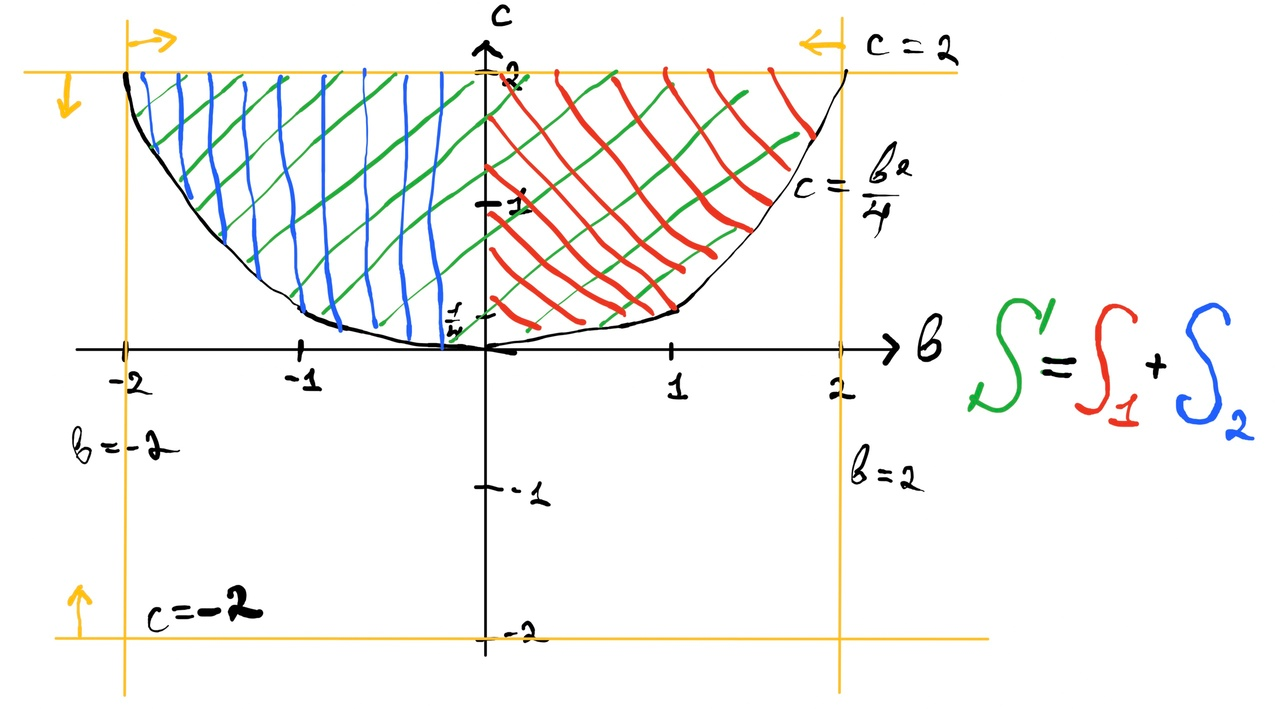
\includegraphics[width=1\linewidth]{geometric_probability}
			\caption{Геометрическая вероятность}
			\label{fig:geometricprobability}
		\end{figure}
		
		
		
		Площадь фигуры, ограниченной неравенствами $-2 \le b, c \le 2$ и $c > \frac{b^2}{4}$, заштрихуем и обозначим через $S$.
		Очевидно, функция $c = \frac{b^2}{4}$ симметрична относительно прямой $b=0$, поэтому исходная площадь  является суммой левой и правой площадей -- $S_1$ и  $S_2$ соответственно, причем $S = S_1 + S_2, \;\; S_1  = S_2$.
		
		Найдем площадь $S_1$ -- она равна разности площади квадрата со стороной 2 и площади под графиком функции $c=\frac{b^2}{4}$ :
		$$S_1 = 2 \cdot 2 - \int_{0}^{2} \frac{b^2}{4} db = 4 - \int_{0}^{2} \frac{x^2}{4} dx = 4 - \frac{1}{4} \int_{0}^{2} x^2 dx = 4 - \frac{1}{4} \frac{x^3}{3} \Bigg|_{0}^{2} = $$
		$$ = 4 - \frac{1}{12} \left(2^3 - 0 \right) = 4 - \frac{1}{12}\cdot 8 = 4 - \frac{8}{12} = 4 - \frac{2}{3} = \frac{10}{3}$$
		
		Тогда $S = S_1 + S_2 = 2 \cdot S_1 = 2 \cdot \frac{10}{3} = \frac{20}{3}$, а общая площадь квадрата $S_{\textit{square}}$ равна $4 \cdot 4 = 16$.
		
		Тогда по геометрической вероятности, вероятность $p$ того, что корни окажутся мнимыми, равна:
		$$p = \frac{S}{S_{\textit{square}}} = \frac{\frac{20}{3}}{16} = \frac{20}{3}\cdot \frac{1}{16} = \frac{20}{3 \cdot 16} = \frac{5}{12}$$
		
		Таким образом, вероятность того, что корни окажутся мнимыми, равна $\frac{5}{12}$.		
\end{proof}
	
\end{document}